\clearpage
\section{KIẾN TRÚC PHẦN CỨNG BKIT ARM4}

\subsection{Nền tảng Phần cứng BKIT ARM4 và Kiến trúc Tổng thể}
Hệ thống điều khiển thang máy 7 tầng được thiết kế lấy bo mạch thí nghiệm \textbf{BKIT ARM4} làm nút xử lý thời gian thực trung tâm, khai thác trực tiếp 13 cụm ngoại vi tích hợp sẵn trên kit mà không cần lắp thêm mạch phụ trợ bên ngoài. Các thông số kiến trúc phần cứng cốt lõi gồm:
\begin{itemize}[nosep]
    \item \textbf{Vi điều khiển trung tâm \texttt{STM32F407ZGT6}:} Sử dụng nhân \textbf{ARM Cortex-M4F} có khối tính toán dấu chấm động phần cứng (\textit{FPU}), hoạt động ở tần số xung nhịp hệ thống \texttt{168~MHz} (bus ngoại vi \texttt{APB1 = 42~MHz}, \texttt{APB2 = 84~MHz}), trang bị \texttt{1~MB Flash}, \texttt{192~KB SRAM} và đóng gói kiểu chân \texttt{LQFP144} với 9 cổng GPIO (\texttt{GPIOA..GPIOI}).
    \item \textbf{Tổ chức 4 phân hệ phần cứng đồng bộ (Hình~\ref{fig:sys_arch}):} Toàn bộ ngoại vi trên bo mạch được quy hoạch thành bốn khối tách biệt:
    \begin{itemize}[nosep]
        \item \textbf{(1) Phân hệ An toàn \& Chấp hành cách ly quang:} Thu nhận tín hiệu ngắt cứng kẹt cửa \texttt{X0}, dừng khẩn \texttt{X1} (\texttt{PA6/PA7}), ngõ vào \texttt{X2/X3}, điều khiển rơ-le động cơ Lên/Xuống \texttt{Y0/Y1} (\texttt{PE5/PE6}), đèn nhịp \texttt{PE4} và còi cảnh báo \texttt{PWM PF8}.
        \item \textbf{(2) Phân hệ Đo lường tương tự 5 kênh \texttt{ADC1}:} Lấy mẫu 12-bit cảm biến nhiệt \texttt{LM35} (\texttt{PC2}), biến trở giả lập tải trọng \texttt{VR1} (\texttt{PC1}), quang trở \texttt{LDR} (\texttt{PC0}), điện áp nguồn \texttt{PB0} và dòng tải \texttt{PB1}.
        \item \textbf{(3) Phân hệ Bus HMI dùng chung \texttt{SPI1} / Lưu trữ \texttt{I2C1} / Flash \texttt{SPI2}:} Quét 4 LED 7 đoạn cùng 16 phím ma trận 4$\times$4 qua \texttt{SPI1}; giao tiếp đồng hồ thời gian thực \texttt{DS3231} (\texttt{0x68}) và hộp đen \texttt{AT24C512} (\texttt{0x50}) qua \texttt{I2C1}; truy xuất Flash \texttt{W25Q64FV} qua \texttt{SPI2}.
        \item \textbf{(4) Phân hệ Truyền thông phân tán \texttt{CAN1} \& \texttt{USART1 RS232}:} Truyền thông công nghiệp vi sai \texttt{bxCAN1} tốc độ \texttt{500~kbps} qua IC \texttt{TJA1050} (\texttt{PB8/PB9}) giữa tủ cabin và sảnh tầng, đồng thời giao tiếp PC Shell CLI và luồng \texttt{\$TWIN} qua \texttt{USART1} (\texttt{PA9/PA10}).
    \end{itemize}
    \item \textbf{Định vị vật lý trên bo mạch thực tế (Hình~\ref{fig:bkit_map}):} Vị trí chính xác của 13 cụm linh kiện ngoại vi cùng 4 cụm công tắc gạt DIP Switch (\texttt{SW2, SW11, SW12, SW13}) phục vụ công tác đấu nối, kiểm tra tín hiệu và trình diễn được đánh dấu trực quan trên sơ đồ bo mạch thật.
    \item \textbf{Phân hoạch bộ nhớ, định thời hệ thống và cơ chế bảo vệ phần cứng:} Tổng dung lượng firmware biên dịch chỉ chiếm \texttt{104\,112~Bytes} (\texttt{9.93\%} Flash) và \texttt{28\,608~Bytes} (\texttt{21.83\%} SRAM chính \texttt{128~KB}, còn nguyên \texttt{64~KB CCM}). Hệ thống tích hợp bộ giám sát độc lập \textbf{IWDG} (\texttt{2500~ms}), bộ đếm chu kỳ phần cứng \texttt{DWT} (\texttt{168~MHz}) đo trực tiếp độ trễ ngắt \texttt{EXTI}, cùng cổng nạp/gỡ lỗi \textbf{ST-LINK} (\texttt{SWD}).
\end{itemize}
Nhờ cách tổ chức phân tách rạch ròi giữa tầng cách ly quang công nghiệp, đường truyền vi sai \texttt{CAN} và các bus chia sẻ \texttt{SPI1/I2C1} ở mức phần cứng, bo mạch \textbf{BKIT ARM4} vừa khai thác tối đa ngoại vi tích hợp sẵn vừa bảo đảm độ tin cậy và thời hạn đáp ứng an toàn dưới \texttt{1~ms} (chi tiết bố trí linh kiện ở Hình~\ref{fig:bkit_map} và sơ đồ khối ở Hình~\ref{fig:sys_arch}).



\begin{figure}[H]
\centering
\resizebox{\textwidth}{!}{%
\begin{tikzpicture}
    % === KHOI MCU TRUNG TAM (STM32F407ZGT6 - LQFP144) ===
    \draw[draw=tablehead, fill=tablehead!3, line width=1.1pt] (-3.75, -5.65) rectangle (3.75, 6.05);
    \draw[draw=tablehead, fill=tablehead!12, line width=0.8pt] (-3.75, 5.00) rectangle (3.75, 6.05);
    \node[align=center, font=\footnotesize\bfseries, text=tablehead] at (0, 5.52)
        {STM32F407ZGT6 (\texttt{LQFP144})\\[1pt]{\tiny\normalfont ARM Cortex-M4F @ 168 MHz | 1 MB Flash | 192 KB SRAM}};

    % Lop phan mem ben trong MCU (4 dong gon -> khong cham AHB1)
    \node[acadbox, text width=6.7cm, fill=white, minimum height=1.25cm] (sw_core) at (0, 3.90)
        {\textbf{Zephyr RTOS v4.4.0 (7 Luồng tĩnh)}\\[1pt]
         {\tiny P2..P8: An toàn $\cdot$ HSM $\cdot$ CAN $\cdot$ HMI $\cdot$ Watchdog}\\
         {\tiny HSM 9 Trạng thái $\cdot$ Lập lịch \texttt{SCAN/LOOK} $\cdot$ Khóa liên động Core}};

    % Cac bo dieu khien ngoai vi ben trong MCU (buoc doc 1.85cm rong rai)
    \node[acadport, minimum width=2.85cm] (p_gpioin)  at (-1.95, 1.35)  {EXTI6/7 \& GPIOA/C};
    \node[acadport, minimum width=2.85cm] (p_gpioout) at (-1.95, -0.50) {GPIOE Out \& DWT};
    \node[acadport, minimum width=2.85cm] (p_tim13)   at (-1.95, -2.35) {TIM13\_CH1 (PWM)};
    \node[acadport, minimum width=2.85cm] (p_adc1)    at (-1.95, -4.20) {ADC1 (12-bit SAR)};

    \node[acadport, minimum width=2.85cm] (p_spi1)    at (1.95, 1.35)   {SPI1 (Mutex Bus)};
    \node[acadport, minimum width=2.85cm] (p_spi2)    at (1.95, -0.50)  {SPI2 Master};
    \node[acadport, minimum width=2.85cm] (p_i2c1)    at (1.95, -2.35)  {I2C1 (Mutex Bus)};
    \node[acadport, minimum width=2.85cm] (p_usart1)  at (1.95, -4.20)  {USART1 UART};

    % Bo dieu khien day MCU: CAN1 & IWDG
    \node[acadport, minimum width=2.85cm] (p_can1)    at (-1.85, -5.20) {bxCAN1 (500 kbps)};
    \node[acadport, minimum width=2.85cm] (p_iwdg)    at (1.85, -5.20)  {IWDG (2500 ms) \& SWD};

    % Bus noi bo ben trong MCU
    \draw[acadline, line width=1.1pt] (0, 2.95) -- (0, -4.65);
    \node[acadlbl, font=\tiny\bfseries] at (0, 2.30) {AHB1 / APB1 / APB2};
    \foreach \y in {1.35, -0.50, -2.35, -4.20} {
        \draw[acadline] (-0.48, \y) -- (0.48, \y);
        \fill (0, \y) circle (1.3pt);
    }
    \draw[acadline] (0, -4.65) -| (p_can1.north);
    \draw[acadline] (0, -4.65) -| (p_iwdg.north);

    % === NGOAI VI BEN TRAI (dat o x=-8.75 -> mep phai khung zone o ~-6.08, cach MCU -3.75 toi 2.33cm!) ===
    \node[acadbox, text width=4.70cm, minimum height=1.20cm] (ext_in) at (-8.75, 1.35)
        {\textbf{Ngõ vào Cách ly Quang \texttt{X0..X3}}\\[1pt]
         {\tiny \texttt{X0(PA6)}: Kẹt cửa $\cdot$ \texttt{X1(PA7)}: E-Stop}\\
         {\tiny \texttt{X2(PC4)}: Tầng $\cdot$ \texttt{X3(PC5)}: Quá tải số}};

    \node[acadbox, text width=4.70cm, minimum height=1.20cm] (ext_out) at (-8.75, -0.50)
        {\textbf{Ngõ ra Rơ-le Quang \texttt{Y0, Y1, LED3}}\\[1pt]
         {\tiny \texttt{Y0(PE5)}: Động cơ LÊN $\cdot$ \texttt{Y1(PE6)}: XUỐNG}\\
         {\tiny \texttt{PE4}: Đèn Heartbeat RTOS}};

    \node[acadbox, text width=4.70cm, minimum height=1.05cm] (ext_pwm) at (-8.75, -2.35)
        {\textbf{Còi Cảnh báo PWM (\texttt{PF8})}\\[1pt]
         {\tiny Tần số \texttt{1.5..3.0 kHz} (50\% duty, non-block)}};

    \node[acadbox, text width=4.70cm, minimum height=1.20cm] (ext_adc) at (-8.75, -4.20)
        {\textbf{Cảm biến Tương tự (5 kênh \texttt{ADC1})}\\[1pt]
         {\tiny \texttt{LM35(PC2)} $\cdot$ \texttt{VR1(PC1)} $\cdot$ \texttt{LDR(PC0)}}\\
         {\tiny Áp nguồn \texttt{PB0} $\cdot$ Dòng tải \texttt{PB1}}};

    % Duong noi ben trai (nhan nam hoan toan trong khoang trang giua zone va MCU: x = -4.92)
    \draw[acadarr] (ext_in.east) -- (-3.75, 1.35);
    \node[acadlbl, anchor=south] at (-4.92, 1.39) {4 bit Active-Low};
    \draw[acadarr] (-3.75, -0.50) -- (ext_out.east);
    \node[acadlbl, anchor=south] at (-4.92, -0.46) {3 đường \texttt{PE4..6}};
    \draw[acadarr] (-3.75, -2.35) -- (ext_pwm.east);
    \node[acadlbl, anchor=south] at (-4.92, -2.31) {\texttt{PF8 (AF9)}};
    \draw[acadarr] (ext_adc.east) -- (-3.75, -4.20);
    \node[acadlbl, anchor=south] at (-4.92, -4.16) {5 kênh ($0..3.3\text{V}$)};

    % === NGOAI VI BEN PHAI (dat o x=+8.80 -> mep trai khung zone o ~+6.10, cach MCU +3.75 toi 2.35cm!) ===
    \node[acadbox, text width=4.75cm, minimum height=1.20cm] (ext_spi1) at (8.80, 1.35)
        {\textbf{Giao diện HMI (\texttt{Shared SPI1}, 1 MHz)}\\[1pt]
         {\tiny 2$\times$\texttt{74HC595}(\texttt{PG6}): 4 LED 7 đoạn \texttt{UP/dn}}\\
         {\tiny 2$\times$\texttt{74HC165}(\texttt{PD3}): Ma trận 16 phím 4$\times$4}};

    \node[acadbox, text width=4.75cm, minimum height=1.05cm] (ext_spi2) at (8.80, -0.50)
        {\textbf{Bộ nhớ NOR Flash \texttt{W25Q64FV}}\\[1pt]
         {\tiny 8 MB (\texttt{SPI2 PB12..15}, JEDEC \texttt{EF 40 17})}};

    \node[acadbox, text width=4.75cm, minimum height=1.20cm] (ext_i2c1) at (8.80, -2.35)
        {\textbf{Lưu trữ \& Giờ thực (\texttt{Shared I2C1})}\\[1pt]
         {\tiny \texttt{DS3231 RTC} (\texttt{0x68}): Giờ thực BCD}\\
         {\tiny \texttt{AT24C512 EEPROM} (\texttt{0x50}): Hộp đen 32 ô}};

    \node[acadbox, text width=4.75cm, minimum height=1.20cm] (ext_uart) at (8.80, -4.20)
        {\textbf{\texttt{MAX3232} $\leftrightarrow$ PC Twin / HIL}\\[1pt]
         {\tiny \texttt{USART1 RS232 DB9} (\texttt{115200 8N1})}\\
         {\tiny Zephyr Shell CLI \& \texttt{\$TWIN} 200ms}};

    % Duong noi ben phai (nhan nam hoan toan trong khoang trang giua MCU va zone: x = +4.95)
    \draw[acadbiarr] (3.75, 1.35) -- (ext_spi1.west);
    \node[acadlbl, anchor=south] at (4.95, 1.39) {\texttt{PB3..5, PG6, PD3}};
    \draw[acadbiarr] (3.75, -0.50) -- (ext_spi2.west);
    \node[acadlbl, anchor=south] at (4.95, -0.46) {\texttt{PB12..15} (2 MHz)};
    \draw[acadbiarr] (3.75, -2.35) -- (ext_i2c1.west);
    \node[acadlbl, anchor=south] at (4.95, -2.31) {\texttt{PB6/7} (400 kHz)};
    \draw[acadbiarr] (3.75, -4.20) -- (ext_uart.west);
    \node[acadlbl, anchor=south] at (4.95, -4.16) {\texttt{PA9/PA10} TX/RX};

    % === NGOAI VI PHIA DUOI (CAN1 TJA1050 & ST-LINK) ===
    \node[acadbox, text width=5.3cm, minimum height=1.05cm] (ext_can) at (-3.45, -7.25)
        {\textbf{Bộ thu phát Vi sai \texttt{TJA1050} (\texttt{SW13=ON})}\\[1pt]
         {\tiny \texttt{CANH / CANL} ($120~\Omega$) $\leftrightarrow$ 1-Kit Loopback / 2-Kit \texttt{CABIN$\leftrightarrow$HALL}}};

    \node[acadbox, text width=4.7cm, minimum height=1.05cm] (ext_stlink) at (3.45, -7.25)
        {\textbf{Mạch Nạp \& Gỡ lỗi \texttt{ST-LINK} (\texttt{SW11=ON})}\\[1pt]
         {\tiny Giao tiếp \texttt{SWDIO / SWCLK} \& Reset MCU}};

    \draw[acadbiarr] (p_can1.south) -- ++(0, -0.75) -| (ext_can.north);
    \node[acadlbl, anchor=south] at (-2.65, -6.18) {\texttt{PB8 / PB9}};
    \draw[acadbiarr] (p_iwdg.south) -- ++(0, -0.75) -| (ext_stlink.north);
    \node[acadlbl, anchor=south] at (2.65, -6.18) {\texttt{SWD}};

    % Khung bao phan he net dut trang nha
    \begin{scope}[on background layer]
        \node[acadzone, fit=(ext_in)(ext_out)(ext_pwm)(ext_adc), label={[font=\tiny\bfseries, text=black!75]above:PHÂN HỆ CẢM BIẾN \& CHẤP HÀNH TẠI CHỖ}] {};
        \node[acadzone, fit=(ext_spi1)(ext_spi2)(ext_i2c1)(ext_uart), label={[font=\tiny\bfseries, text=black!75]above:PHÂN HỆ BUS HMI, LƯU TRỮ \& PC HIL}] {};
    \end{scope}
\end{tikzpicture}%
}

\caption{Sơ đồ khối kiến trúc kết nối phần cứng trung tâm \texttt{STM32F407ZGT6} (BKIT ARM4) và các phân hệ ngoại vi}
\label{fig:sys_arch}
\end{figure}

\begin{figure}[H]
\centering
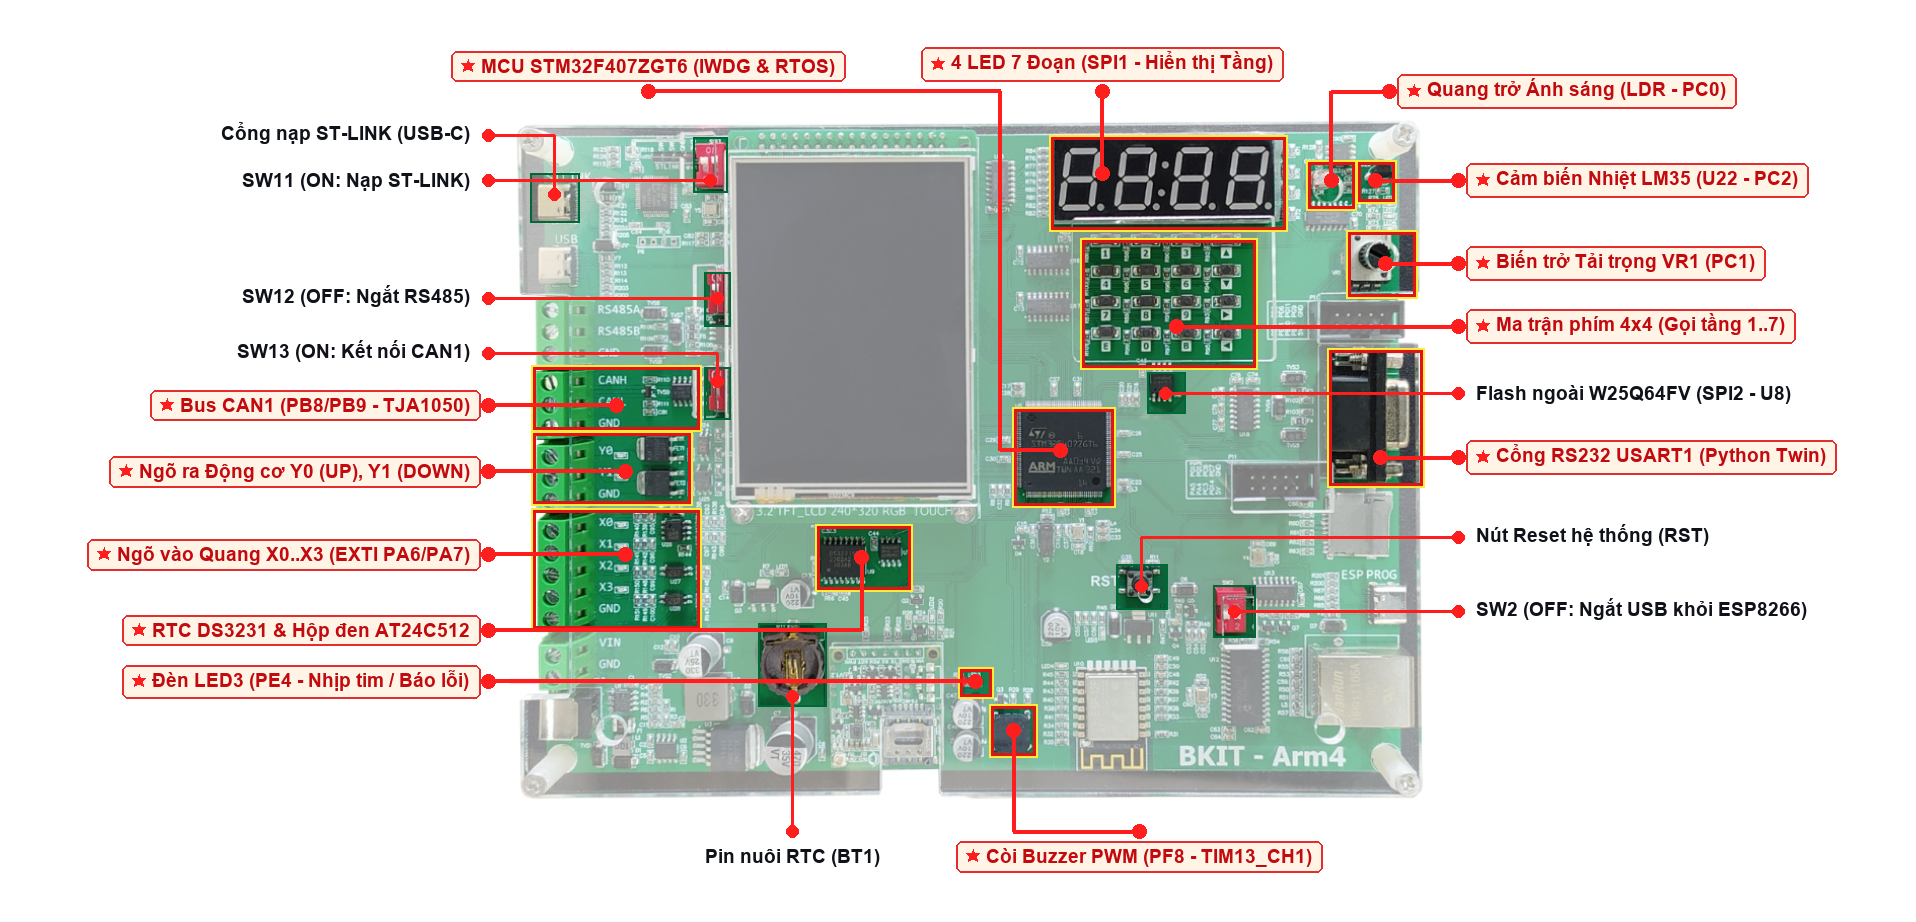
\includegraphics[width=\textwidth]{image/bkit_arm4_project_map.png}
\caption{Sơ đồ định vị thực tế 13 cụm ngoại vi cốt lõi và cấu hình DIP Switch trên bo mạch BKIT ARM4}
\label{fig:bkit_map}
\end{figure}

\newpage
\subsection{Phân tích Nguyên lý Giao tiếp 4 Phân hệ Ngoại vi trên Kit}
Nguyên lý kết nối phần cứng, mức điện áp và cơ chế phân xử bus của 4 phân hệ gồm:

\subsubsection{Phân hệ An toàn Cách ly Quang (\texttt{X0..X3}, \texttt{Y0..Y1}) và Còi xung \texttt{PWM PF8}}
\begin{itemize}[nosep]
    \item \textbf{Ngõ vào cách ly quang \texttt{Opto In X0..X3} (\texttt{PA6, PA7, PC4, PC5}):}
    \begin{itemize}[nosep]
        \item \textit{Cách ly và mức logic:} Tín hiệu công tắc và cảm biến đi qua tầng ghép quang \textit{optocoupler} giúp cách ly điện áp công nghiệp và chống nhiễu xung khỏi các chân vi điều khiển; ngõ vào cấu hình điện trở kéo lên nội và tích cực mức thấp, giữ mức cao ổn định khi hở mạch.
        \item \textit{Ngắt cứng \texttt{EXTI6/7} (\texttt{X0, X1}):} Hai chân \texttt{X0 (PA6 -- Kẹt cửa)} và \texttt{X1 (PA7 -- E-Stop)} cấu hình ngắt ngoài theo sườn tích cực, lập tức chụp giá trị bộ đếm chu kỳ phần cứng \texttt{DWT} trước khâu lọc rung tiếp điểm \texttt{40~ms} để định lượng độ trễ phần cứng ở mức micro-giây.
        \item \textit{Đọc định kỳ \texttt{X2/X3}:} Chân \texttt{X3 (PC5)} nối công tắc quá tải cơ khí được tác vụ giám sát an toàn lấy mẫu mỗi \texttt{100~ms} và hợp logic (OR) cùng ngưỡng cân \texttt{VR1} ($\ge 800\text{ kg}$), còn \texttt{X2 (PC4)} dự phòng cho cảm biến hành trình tầng.
    \end{itemize}
    \item \textbf{Ngõ ra cách ly quang \texttt{Y0/Y1} (\texttt{PE5/PE6}) và \texttt{LED3} (\texttt{PE4}):}
    \begin{itemize}[nosep]
        \item \textit{Điều khiển động cơ kéo:} Hai ngõ ra tích cực mức cao cách ly quang để kích rơ-le chiều \textbf{LÊN (\texttt{Y0 -- PE5})} và \textbf{XUỐNG (\texttt{Y1 -- PE6})}; mạch và logic điều khiển luôn áp dụng khóa liên động kép, tự động ngắt cả hai chân về mức \texttt{0} nếu xuất hiện lệnh xung đột.
        \item \textit{Đèn nhịp hệ thống (\texttt{PE4}):} \texttt{LED3} đóng vai đèn nhịp giám sát trực quan trạng thái vận hành, nháy chậm chu kỳ \texttt{800~ms} khi cabin làm việc bình thường và chuyển sang nháy nhanh \texttt{200~ms} ngay khi hệ thống phát sinh báo cháy hoặc sự cố an toàn.
    \end{itemize}
    \item \textbf{Còi cảnh báo \texttt{PWM PF8} (\texttt{TIM13\_CH1}):}
    \begin{itemize}[nosep]
        \item \textit{Cấu hình bộ định thời:} Chân \texttt{PF8} được ánh xạ sang chức năng thay thế \texttt{AF9} nối với \texttt{TIM13\_CH1}; xung nhịp timer trên bus \texttt{APB1} đạt \texttt{84~MHz}, qua bộ chia tần \texttt{/84} tạo chuẩn đếm \texttt{1~MHz} ($1~\mu\text{s/tick}$) để sinh dải tần chính xác.
        \item \textit{Phát âm không chặn:} Xuất xung vuông chu kỳ nhiệm vụ \texttt{50\%} giúp còi thụ động đạt âm lượng cực đại theo 5 âm báo chuẩn lưu trong Flash (\texttt{1.5..3.0~kHz}), có khóa \textit{mutex} đồng bộ truy cập và tự ngắt theo nhịp định thời không chặn trên tác vụ giao diện.
    \end{itemize}
\end{itemize}

\subsubsection{Phân hệ Đo lường Tương tự 5 Kênh (\texttt{ADC1 12-bit})}
Bộ chuyển đổi \texttt{ADC1} vận hành ở chế độ lấy mẫu đồng bộ, độ phân giải \texttt{12-bit} ($0..4095$) với điện áp tham chiếu nội ($V_{\text{REF}} = 3300\text{ mV}$, bước lượng tử $V_{\text{LSB}} \approx 0.806\text{ mV}$), độ lợi $1\times$ và bộ chia xung nhịp \texttt{/4}:
\begin{itemize}[nosep]
    \item \textbf{Cảm biến nhiệt độ \texttt{LM35} (\texttt{PC2 -- ADC1\_IN12}):} Tuân theo đặc tuyến tuyến tính chuẩn $10\text{ mV}/^\circ\text{C}$, được quy đổi trực tiếp từ điện áp \texttt{mV} sang đơn vị nguyên $0.1^\circ\text{C}$ ($1\text{ mV} \equiv 0.1^\circ\text{C}$, số học dấu phẩy tĩnh), tránh chi phí dấu phẩy động mà vẫn bảo đảm theo dõi chính xác ngưỡng cháy $55.0^\circ\text{C}/48.0^\circ\text{C}$.
    \item \textbf{Biến trở tải trọng \texttt{VR1} (\texttt{PC1 -- ADC1\_IN11}):} Quy đổi tuyến tính dải điện áp $0..3300\text{ mV}$ theo tỉ lệ $m_{\text{kg}} = (V_{\text{VR1}} / 3300) \times 1000\text{ kg}$ thành tải trọng giả lập $0..1000\text{ kg}$ thay thế \textit{loadcell}, kết hợp trễ hồi (\textit{hysteresis}) để chặn đóng cửa khi vượt ngưỡng $800\text{ kg}/750\text{ kg}$.
    \item \textbf{Ba kênh đo giám sát bổ trợ (\texttt{PC0, PB0, PB1}):} Thu nhận trực tiếp điện áp \texttt{mV} ($0..3300\text{ mV}$) từ quang trở \texttt{LDR (PC0 -- IN10)}, kênh đo áp nguồn bus (\texttt{PB0 -- IN8}) và dòng tải (\texttt{PB1 -- IN9}), phục vụ tự kiểm tra độ ổn định mạch tương tự và xuất thông số chẩn đoán qua giao diện dòng lệnh trên UART.
\end{itemize}

\subsubsection{Phân hệ Bus Dùng chung \texttt{SPI1}, \texttt{I2C1} và NOR Flash \texttt{SPI2}}
Đây là cụm ngoại vi chia sẻ bus vật lý, đòi hỏi đồng bộ chặt chẽ ở cả tầng phần cứng lẫn hệ điều hành thời gian thực (Hình~\ref{fig:shared_buses}):
\begin{itemize}[nosep]
    \item \textbf{Bus \texttt{SPI1} dùng chung (\texttt{PB3 SCK}, \texttt{PB4 MISO}, \texttt{PB5 MOSI}, \texttt{1~MHz}):}
    \begin{itemize}[nosep]
        \item \textit{Nhánh xuất LED 7 đoạn:} Sử dụng \textbf{2 $\times$ \texttt{74HC595}} mắc nối tiếp nhận \texttt{16-bit} dữ liệu (byte mã đoạn \texttt{a..g} và byte chọn vị trí LED) truyền bit có trọng số cao trước (\textit{MSB-first}), chốt đồng loạt bằng xung sườn lên \texttt{2~$\mu$s} trên chân \texttt{PG6 (LD\_LATCH)} ở tần số quét \texttt{100~Hz} để hiển thị tầng, mũi tên \texttt{UP/dn}, \texttt{FE} và \texttt{Err}.
        \item \textit{Nhánh nhập ma trận phím 4$\times$4:} Sử dụng \textbf{2 $\times$ \texttt{74HC165}} đọc 16 phím tích cực mức thấp; trước mỗi lượt quét chu kỳ \texttt{50~ms}, vi điều khiển phát xung nạp song song qua chân \texttt{PD3 (BTN\_LOAD)} rồi dịch 2 byte về \texttt{MISO (PB4)}, tự động lọc bỏ trạng thái nghỉ (\texttt{0xFFFF}) và nhiễu thả nổi (\texttt{0x0000}).
        \item \textit{Phân xử bus:} Do hai mạch thanh ghi dịch dùng chung đường xung nhịp \texttt{SCK (PB3)}, mọi giao dịch trên \texttt{SPI1} đều được tuần tự hóa bằng khóa \textit{mutex} phân xử bus có kế thừa độ ưu tiên (\textit{Priority Inheritance}), ngăn chặn hoàn toàn hiện tượng lem LED hay sai mã phím khi tác vụ quét đồng thời.
    \end{itemize}
    \item \textbf{Bus \texttt{I2C1} dùng chung (\texttt{PB6 SCL}, \texttt{PB7 SDA}, \textit{Fast-Mode} \texttt{400~kHz}):}
    \begin{itemize}[nosep]
        \item \textit{Đồng hồ \texttt{DS3231 RTC} (\texttt{0x68}):} Tích hợp pin dự phòng CR2032 giúp duy trì giờ chuẩn ngay cả khi mất nguồn chính; vi điều khiển đọc liên tiếp các thanh ghi \texttt{0x00..0x06} và giải mã từ dạng nhị phân thập phân (\texttt{BCD}) sang nhị phân thuần để gắn dấu thời gian cho từng bản ghi sự cố.
        \item \textit{Hộp đen \texttt{AT24C512 EEPROM} (\texttt{0x50}):} Dung lượng \texttt{64~KB} (\texttt{65\,536 Bytes}) tổ chức theo trang \texttt{128 Bytes}; vùng đầu (\texttt{0x0000}) lưu khối tiêu đề kiểm tra \texttt{CRC32}, còn vùng dữ liệu (\texttt{0x0080}) lưu bộ đệm vòng 32 bản ghi bước \texttt{32 Bytes} kèm \texttt{CRC16} nhằm bảo toàn nhật ký khi mất điện mà không ghi vượt ranh giới trang.
        \item \textit{Phân xử bus:} Hai thiết bị dùng chung đường truyền cực máng hở \texttt{PB6/PB7} nối điện trở kéo lên $R_{p1}, R_{p2}$ về nguồn \texttt{+3.3~V}, đồng thời mọi thao tác đọc/ghi thời gian hay hộp đen đều được tuần tự hóa qua khóa \textit{mutex} riêng của bus \texttt{I2C1} để tránh xung đột khung truyền.
    \end{itemize}
    \newpage
    \item \textbf{Bus \texttt{SPI2} độc lập (\texttt{PB12..PB15}, \texttt{2~MHz}):}
    \begin{itemize}[nosep]
        \item \textit{NOR Flash \texttt{W25Q64FV} (\texttt{8~MB}):} Vận hành trên bus \texttt{SPI2} tách biệt qua chân chọn chip \texttt{PB12} tích cực mức thấp nên không tranh chấp băng thông với nhánh HMI; khi khởi tạo hoặc kiểm tra phần cứng, firmware phát lệnh \texttt{0x9F} đọc về mã \texttt{JEDEC ID 0xEF 0x40 0x17} xác nhận kết nối.
    \end{itemize}
\end{itemize}

\begin{figure}[H]
\centering
\resizebox{\textwidth}{!}{%
\begin{tikzpicture}
    % ==================== NUA TRAI: SHARED SPI1 ====================
    \draw[draw=black!55, dashed, fill=black!2, line width=0.6pt] (-0.3, -4.55) rectangle (9.05, 3.65);
    \node[font=\footnotesize\bfseries, text=tablehead, anchor=west] at (-0.1, 3.30) {(a) Kiến trúc Bus \texttt{SPI1} Dùng chung (1 MHz)};

    % MCU SPI1 Master
    \node[acadmcu, text width=2.55cm, minimum height=4.8cm] (mcu_spi) at (1.30, -0.20)
        {\textbf{STM32F407}\\[-1pt]\texttt{SPI1 Master}\\[6pt]
         {\tiny Bộ phân xử:}\\[-1pt]
         {\tiny\textbf{Mutex Bus SPI1}}\\[-1pt]
         {\tiny (\textit{Priority Inheritance})}};

    % 2x 74HC595 + 4 LED 7 doan
    \node[acadbox, text width=3.10cm, minimum height=1.85cm] (hc595) at (7.20, 1.45)
        {\textbf{2 $\times$ IC \texttt{74HC595}}\\[-1pt]
         {\tiny Ghi dịch SIPO (16-bit)}\\[-1pt]
         {\tiny $\rightarrow$ \textbf{4 LED 7 đoạn Anode chung}}\\[-1pt]
         {\tiny Hiển thị \texttt{UP/dn}, \texttt{FE}, \texttt{Err} @ 100 Hz}};

    % 2x 74HC165 + Ma tran 16 phim
    \node[acadbox, text width=3.10cm, minimum height=1.85cm] (hc165) at (7.20, -1.95)
        {\textbf{2 $\times$ IC \texttt{74HC165}}\\[-1pt]
         {\tiny Ghi dịch PISO (16-bit)}\\[-1pt]
         {\tiny $\leftarrow$ \textbf{Ma trận 16 phím 4$\times$4}}\\[-1pt]
         {\tiny Active-Low (\texttt{0..15}, \texttt{0xFFFF}=idle)}};

    % Dau noi day bus SPI1 (kenh day rong ~2.7cm, nhan can giua khoang trong, tach hoan toan vien hop)
    \draw[acadarr] (mcu_spi.east |- 0, 1.95) -- node[acadpin, above=1.5pt, pos=0.44] {\texttt{PB3 (SCK)}} (hc595.west |- 0, 1.95);
    \draw[acadarr] (5.12, 1.95) |- ($(hc165.west)+(0, 0.50)$);
    \fill (5.12, 1.95) circle (1.4pt);

    \draw[acadarr] (mcu_spi.east |- 0, 1.25) -- node[acadpin, above=1.5pt, pos=0.44] {\texttt{PB5 (MOSI)}} (hc595.west |- 0, 1.25);
    \draw[acadarr] (hc165.west |- 0, -1.25) -- node[acadpin, above=1.5pt, pos=0.50] {\texttt{PB4 (MISO)}} (mcu_spi.east |- 0, -1.25);

    \draw[acadarr, draw=tablehead] (mcu_spi.east |- 0, 0.58) -- node[acadpin, above=1.5pt, pos=0.48] {\texttt{PG6 (LD\_LATCH)}} (hc595.west |- 0, 0.58);
    \draw[acadarr, draw=tablehead] (mcu_spi.east |- 0, -2.45) -- node[acadpin, above=1.5pt, pos=0.50] {\texttt{PD3 (BTN\_LOAD)}} (hc165.west |- 0, -2.45);

    \node[font=\tiny\itshape, align=center, text=black!80] at (4.35, -3.95)
        {Lưu ý: Tác vụ HMI khóa \textbf{Mutex Bus SPI1} trước khi tạo xung \texttt{PG6} hoặc \texttt{PD3},\\
         loại bỏ hoàn toàn nhiễu bấm phím làm nhòe LED 7 đoạn.};

    % ==================== NUA PHAI: SHARED I2C1 ====================
    \draw[draw=black!55, dashed, fill=black!2, line width=0.6pt] (9.35, -4.55) rectangle (19.15, 3.65);
    \node[font=\footnotesize\bfseries, text=tablehead, anchor=west] at (9.55, 3.30) {(b) Kiến trúc Bus \texttt{I2C1} Dùng chung (400 kHz)};

    % MCU I2C1 Master
    \node[acadmcu, text width=2.45cm, minimum height=4.2cm] (mcu_i2c) at (10.85, -0.35)
        {\textbf{STM32F407}\\[-1pt]\texttt{I2C1 Master}\\[6pt]
         {\tiny Bộ phân xử:}\\[-1pt]
         {\tiny\textbf{Mutex Bus I2C1}}\\[-1pt]
         {\tiny (\textit{Priority Inheritance})}};

    % Nguon 3.3V va dien tro keo len Rp (tach xa vien MCU va day doc bus I2C)
    \node[font=\tiny\bfseries] (vcc) at (14.40, 2.58) {\texttt{+3.3V}};
    \draw[acadline] (13.70, 2.33) -- (15.10, 2.33);
    % Rp1 SCL
    \draw[acadline] (14.00, 2.33) -- (14.00, 1.98);
    \draw[acadline, fill=white] (13.89, 1.43) rectangle (14.11, 1.98);
    \draw[acadline] (14.00, 1.43) -- (14.00, 0.85);
    \node[font=\tiny] at (13.60, 1.70) {$R_{p1}$};
    % Rp2 SDA
    \draw[acadline] (14.80, 2.33) -- (14.80, 1.98);
    \draw[acadline, fill=white] (14.69, 1.43) rectangle (14.91, 1.98);
    \draw[acadline] (14.80, 1.43) -- (14.80, 0.05);
    \node[font=\tiny] at (15.20, 1.70) {$R_{p2}$};

    % Duong bus SCL & SDA (nhan dat cach xa mep phai MCU >= 2.5mm)
    \draw[acadarr] (mcu_i2c.east |- 0, 0.85) -- (15.72, 0.85);
    \node[acadpin, anchor=south west] at (12.48, 0.90) {\texttt{PB6(SCL)}};
    \draw[acadbiarr] (mcu_i2c.east |- 0, 0.05) -- (15.72, 0.05);
    \node[acadpin, anchor=south west] at (12.48, 0.10) {\texttt{PB7(SDA)}};
    \fill (14.00, 0.85) circle (1.4pt);
    \fill (14.80, 0.05) circle (1.4pt);

    % 2 IC tren I2C1: DS3231 & AT24C512
    \node[acadbox, text width=2.85cm, minimum height=1.75cm] (ds3231) at (17.45, 1.45)
        {\textbf{IC \texttt{DS3231 RTC}}\\[-1pt]
         {\tiny Địa chỉ 7-bit: \texttt{0x68}}\\[-1pt]
         {\tiny Pin dự phòng CR2032}\\[-1pt]
         {\tiny Cung cấp giờ thực BCD}};

    \node[acadbox, text width=2.85cm, minimum height=1.95cm] (at24) at (17.45, -1.75)
        {\textbf{IC \texttt{AT24C512 EEPROM}}\\[-1pt]
         {\tiny Địa chỉ 7-bit: \texttt{0x50}}\\[-1pt]
         {\tiny 64 KB (Trang 128 B)}\\[-1pt]
         {\tiny Hộp đen 32 ô \texttt{CRC16/32}}};

    % Nhanh re xuong DS3231 & AT24C512 (o x=15.55 cach xa Rp2 o 15.20)
    \draw[acadline] (15.55, 0.85) |- ($(ds3231.west)+(0, 0.30)$);
    \draw[acadline] (15.55, 0.05) |- ($(ds3231.west)+(0, -0.30)$);
    \draw[acadline] (15.55, 0.85) |- ($(at24.west)+(0, 0.35)$);
    \draw[acadline] (15.55, 0.05) |- ($(at24.west)+(0, -0.25)$);
    \fill (15.55, 0.85) circle (1.4pt);
    \fill (15.55, 0.05) circle (1.4pt);

    \node[font=\tiny\itshape, align=center, text=black!80] at (14.25, -3.95)
        {Lưu ý: Loại bỏ \texttt{\&audio\_codec CS43L22} và chuyển \texttt{\&i2c1} về \texttt{PB6/PB7}\\
         giúp giải phóng hoàn toàn chân \texttt{PB9} cho bộ thu phát \texttt{CAN1\_TX}.};
\end{tikzpicture}%
}

\caption{Sơ đồ nguyên lý ghép nối và phân xử bus dùng chung \texttt{SPI1} (\texttt{74HC595} / \texttt{74HC165}) và \texttt{I2C1} (\texttt{DS3231} / \texttt{AT24C512})}
\label{fig:shared_buses}
\end{figure}

\subsubsection{Phân hệ Truyền thông Phân tán \texttt{CAN1} và Giao tiếp \texttt{USART1 RS232}}
\begin{itemize}[nosep]
    \item \textbf{Mạng \texttt{bxCAN1} tốc độ \texttt{500~kbps} (\texttt{PB8 CAN1\_RX}, \texttt{PB9 CAN1\_TX}):}
    \begin{itemize}[nosep]
        \item \textit{Giao tiếp vi sai chống nhiễu:} Bộ điều khiển \texttt{bxCAN1} chuẩn \texttt{CAN 2.0A} (ID 11-bit) xuất tín hiệu qua bộ thu phát vi sai \textbf{\texttt{TJA1050}} (đóng \texttt{SW13 = ON}) ra cặp dây \texttt{CANH / CANL} có trở đầu cuối \texttt{120~$\Omega$}, điểm lấy mẫu $87.5\%$ chu kỳ bit giúp miễn nhiễu công nghiệp.
        \item \textit{Chế độ vận hành linh hoạt:} Chuyển đổi linh hoạt giữa tự kiểm 1 kit (\texttt{LOOPBACK}) và nối mạng 2 kit (\texttt{NORMAL}: \texttt{CABIN} $\leftrightarrow$ \texttt{HALL}); bộ lọc phần cứng thu hẹp 3 dải ID trọng yếu (\texttt{0x080}, \texttt{0x100..0x10F}, \texttt{0x200..0x3FF}), hỗ trợ khung \texttt{RTR} và giám sát \texttt{TEC/REC} kèm cơ chế phục hồi lỗi bus.
    \end{itemize}
    \item \textbf{Cổng nối tiếp \texttt{USART1 RS232} (\texttt{PA9 TX}, \texttt{PA10 RX}, \texttt{115200 8N1}):}
    \begin{itemize}[nosep]
        \item \textit{Tầng chuyển mức:} Chuyển đổi mức áp \texttt{3.3~V TTL} sang chuẩn đối xứng RS232 qua IC \textbf{\texttt{MAX3232}} ra đầu DB9 về máy tính; gạt \texttt{SW12 = OFF} để cô lập hoàn toàn nhánh RS485 dùng chung chân truyền nhận.
        \item \textit{Kênh song công Shell \& Telemetry:} Đảm nhiệm đồng thời giao diện dòng lệnh \textbf{Zephyr Shell CLI} phục vụ chẩn đoán ngoại vi và luồng bản tin JSON \texttt{\$TWIN} mỗi \texttt{200~ms} đồng bộ trạng thái thời gian thực lên \textbf{PC Digital Twin}.
    \end{itemize}
\end{itemize}

\clearpage
\subsection{Thiết kế Devicetree (\texttt{app.overlay}) và Giải quyết Xung đột Chân}
Bo mạch \textbf{BKIT ARM4} dùng vi điều khiển \texttt{STM32F407ZGT6} (vỏ \texttt{LQFP144}), trong khi bo chuẩn gần nhất của Zephyr RTOS là \texttt{stm32f4\_disco} (\texttt{STM32F407VGT6}, vỏ \texttt{LQFP100}). Do khác biệt số chân I/O và ngoại vi hàn sẵn trên bo Discovery (âm thanh \texttt{cs43l22@4a}, \texttt{usbotg\_fs}, \texttt{leds}, \texttt{gpio\_keys}), việc giữ nguyên cây thiết bị gốc sẽ gây xung đột chân. Tệp phủ \texttt{app.overlay} được viết để chuyển hướng \texttt{chosen} (\texttt{\&usart1}, \texttt{\&can1}), chuẩn hóa \texttt{aliases} (\texttt{led0..2}, \texttt{sw0..3}, \texttt{watchdog0}, \texttt{eeprom-0}, \texttt{pwm-buzzer}) và xử lý 3 nhóm xung đột chính (Hình~\ref{fig:dt_conflict}):
\begin{enumerate}[nosep]
    \item \textbf{Tách chân \texttt{PA6} khỏi \texttt{\&adc1} để dành cho ngắt cứng \texttt{X0}:}
    \begin{itemize}[nosep]
        \item \textit{Xung đột gốc:} Trên \texttt{stm32f4\_disco}, \texttt{pinctrl-0} mặc định của \texttt{\&adc1} ánh xạ cả \texttt{adc1\_in6\_pa6}, trong khi kit \textbf{BKIT ARM4} nối \texttt{PA6} với ngõ vào quang \texttt{X0} đòi hỏi ngắt sườn phát hiện kẹt cửa tức thời.
        \item \textit{Can thiệp \texttt{app.overlay}:} Ghi đè \texttt{pinctrl-0} của \texttt{\&adc1} chỉ giữ 5 kênh (\texttt{PB0, PB1, PC0, PC1, PC2}), khai báo 5 nút \texttt{channel@8..c} (\texttt{12-bit}, \texttt{ADC\_REF\_INTERNAL}, \texttt{SYNC}), tắt \texttt{gpio\_keys} mặc định và gán \texttt{PA6} cho \texttt{bkit\_in\_x0} (\texttt{sw0}).
        \item \textit{Kết quả:} Giải phóng hoàn toàn \texttt{PA6} làm ngắt sườn \texttt{EXTI6} cho cảm biến kẹt cửa \texttt{X0}, tách bạch khỏi chu kỳ quét 5 kênh của \texttt{ADC1}.
    \end{itemize}
    \item \textbf{Tách \texttt{\&i2c1} khỏi chân \texttt{PB9} để giải phóng \texttt{CAN1\_TX}:}
    \begin{itemize}[nosep]
        \item \textit{Xung đột gốc:} Mặc định \texttt{\&i2c1} dùng chân \texttt{i2c1\_sda\_pb9} cho codec âm thanh \texttt{cs43l22@4a}, trùng trực tiếp với chân phát \texttt{CAN1\_TX (PB9)} nối IC \texttt{TJA1050}, đồng thời tồn tại nhiều nút ngoại vi dư thừa dễ tranh chấp chân.
        \item \textit{Can thiệp \texttt{app.overlay}:} Chuyển \texttt{\&i2c1} dùng \texttt{I2C\_BITRATE\_FAST} (\texttt{400~kHz}) tại cặp \texttt{PB6 (SCL) / PB7 (SDA)}, khai báo \texttt{eeprom@50} (\texttt{atmel,at24}, \texttt{64~KB}, trang \texttt{128~B}), tắt các nút \texttt{\&audio\_codec}, \texttt{\&can2}, \texttt{\&usart2}, \texttt{\&i2s3}, \texttt{\&usbotg\_fs}, \texttt{\&timers2/4}, \texttt{leds}, \texttt{pwmleds}; và gán \texttt{\&can1} ra \texttt{PB8/PB9} (\texttt{500~kbps}, \texttt{sample-point = <875>}).
        \item \textit{Kết quả:} Bus vi sai \texttt{bxCAN1} (\texttt{PB8/PB9}) và \texttt{I2C1} (\texttt{PB6/PB7}) phục vụ \texttt{DS3231 RTC} cùng \texttt{AT24C512} vận hành song song không đụng chân.
    \end{itemize}
    \item \textbf{Kích hoạt \texttt{GPIOF/G}, nút \texttt{zephyr,user} và bổ sung \texttt{pinctrl} cho \texttt{PF8}:}
    \begin{itemize}[nosep]
        \item \textit{Giới hạn gốc:} Vỏ \texttt{LQFP100} không khai báo Port F và Port G nên cây thiết bị gốc thiếu định tuyến chân còi \texttt{PF8 (TIM13\_CH1)} và chốt LED 7 đoạn \texttt{PG6 (LD\_LATCH)}.
        \item \textit{Can thiệp \texttt{app.overlay}:} Bật tường minh \texttt{\&gpiof}, \texttt{\&gpiog}, \texttt{\&timers13} (\texttt{st,prescaler = <83>}) và \texttt{\&iwdg}; tạo mới \texttt{tim13\_ch1\_pf8} (\texttt{STM32\_PINMUX('F', 8, AF9)}) cho \texttt{bkit\_buzzer}; đồng thời gom 5 \texttt{io-channels} và 3 chân điều khiển (\texttt{ld-latch-gpios = <\&gpiog 6>}, \texttt{btn-load-gpios = <\&gpiod 3>}, \texttt{w25q-cs-gpios = <\&gpiob 12>}) vào \texttt{zephyr,user}.
        \item \textit{Kết quả:} Khai thác trọn vẹn tài nguyên \texttt{LQFP144} gồm còi \texttt{PWM13 (PF8)}, chốt \texttt{74HC595 (PG6)}, nạp phím \texttt{74HC165 (PD3)} và chọn NOR Flash \texttt{PB12}.
    \end{itemize}
\end{enumerate}

\clearpage
\begin{figure}[H]
\centering
\resizebox{\textwidth}{!}{%
\begin{tikzpicture}
    % Tieu de 3 cot (khop rong voi 3 cot ben duoi, khong bao gio de nhau)
    \node[acadhdr, text width=4.65cm, minimum height=0.68cm] (H1) at (2.5, 4.75)  {TARGET \texttt{stm32f4\_disco} (\texttt{LQFP100})};
    \node[acadhdr, text width=4.85cm, minimum height=0.68cm, fill=tablehead, text=white] (H2) at (8.05, 4.75)  {CAN THIỆP TRONG \texttt{app.overlay}};
    \node[acadhdr, text width=4.85cm, minimum height=0.68cm] (H3) at (13.6, 4.75) {ÁNH XẠ \texttt{BKIT ARM4} (\texttt{LQFP144})};

    % Hang 1: Xung dot PA6
    \node[acadbox, text width=4.65cm, minimum height=1.55cm] (C1L) at (2.5, 3.25)
        {\textbf{Xung đột 1: Chân \texttt{PA6}}\\[1pt]
         {\tiny Mặc định \texttt{\&adc1} gán \texttt{adc1\_in6\_pa6}}\\
         {\tiny $\Rightarrow$ Chiếm dụng chân ngắt cứng \texttt{X0}}};

    \node[acadboxnav, text width=4.85cm, minimum height=1.55cm] (C1M) at (8.05, 3.25)
        {\texttt{\&adc1} ghi đè \texttt{pinctrl-0}:\\[1pt]
         {\tiny Chỉ giữ 5 kênh \texttt{PB0, PB1, PC0, PC1, PC2}}\\
         {\tiny Khai báo \texttt{bkit\_in\_x0: PA6 (ACTIVE\_LOW)}}};

    \node[acadbox, text width=4.85cm, minimum height=1.55cm] (C1R) at (13.6, 3.25)
        {\textbf{\texttt{PA6} $\rightarrow$ Ngắt cứng \texttt{EXTI6} (\texttt{X0})}\\[1pt]
         {\tiny Phát hiện vật cản cửa cabin (tức thời)}\\
         {\tiny Tách bạch hoàn toàn với 5 kênh \texttt{ADC1}}};

    % Hang 2: Xung dot PB9
    \node[acadbox, text width=4.65cm, minimum height=1.55cm] (C2L) at (2.5, 1.30)
        {\textbf{Xung đột 2: Chân \texttt{PB9}}\\[1pt]
         {\tiny Mặc định \texttt{\&i2c1} dùng \texttt{i2c1\_sda\_pb9}}\\
         {\tiny nối codec \texttt{cs43l22@4a} $\Rightarrow$ Đụng \texttt{CAN1\_TX}}};

    \node[acadboxnav, text width=4.85cm, minimum height=1.55cm] (C2M) at (8.05, 1.30)
        {\texttt{\&i2c1} chuyển \texttt{PB6/PB7} (\texttt{400 kHz}):\\[1pt]
         {\tiny Gắn \texttt{status = "disabled"} cho \texttt{\&audio\_codec},}\\
         {\tiny \texttt{\&can2}, \texttt{\&usart2}, \texttt{\&i2s3}, \texttt{\&timers2/4}}};

    \node[acadbox, text width=4.85cm, minimum height=1.55cm] (C2R) at (13.6, 1.30)
        {\textbf{\texttt{PB8/PB9} $\rightarrow$ \texttt{CAN1} | \texttt{PB6/7} $\rightarrow$ \texttt{I2C1}}\\[1pt]
         {\tiny \texttt{bxCAN1} 500 kbps (\texttt{TJA1050}) \& \texttt{DS3231/}}\\
         {\tiny \texttt{AT24C512} chạy đồng thời không xung đột}};

    % Hang 3: Port F va Port G thieu tren LQFP100
    \node[acadbox, text width=4.65cm, minimum height=1.55cm] (C3L) at (2.5, -0.65)
        {\textbf{Xung đột 3: Thiếu Port \texttt{F/G}}\\[1pt]
         {\tiny Vỏ \texttt{LQFP100} không có cổng \texttt{GPIOF/G}}\\
         {\tiny $\Rightarrow$ Không có nút còi \texttt{PF8} \& chốt \texttt{PG6}}};

    \node[acadboxnav, text width=4.85cm, minimum height=1.55cm] (C3M) at (8.05, -0.65)
        {Bật \texttt{\&gpiof}, \texttt{\&gpiog}, \texttt{\&timers13}:\\[1pt]
         {\tiny Khai báo mới \texttt{tim13\_ch1\_pf8 (AF9)}}\\
         {\tiny Gán \texttt{ld-latch-gpios = <\&gpiog 6>}}};

    \node[acadbox, text width=4.85cm, minimum height=1.55cm] (C3R) at (13.6, -0.65)
        {\textbf{\texttt{PF8} $\rightarrow$ \texttt{PWM13} | \texttt{PG6} $\rightarrow$ \texttt{LD\_LATCH}}\\[1pt]
         {\tiny Còi xung PWM đa âm báo (\texttt{TIM13\_CH1})}\\
         {\tiny Chốt dữ liệu 4 LED 7 đoạn qua \texttt{74HC595}}};

    % Mui ten ket noi giua 3 cot
    \foreach \r in {1, 2, 3} {
        \draw[acadarr] (C\r L.east) -- (C\r M.west);
        \draw[acadarr] (C\r M.east) -- (C\r R.west);
    }
\end{tikzpicture}%
}

\caption{Kiến trúc ánh xạ Devicetree giải quyết 3 xung đột phần cứng từ \texttt{stm32f4\_disco} (\texttt{LQFP100}) sang BKIT ARM4 (\texttt{LQFP144})}
\label{fig:dt_conflict}
\end{figure}

Đoạn trích cấu hình từ \texttt{app.overlay} dưới đây minh họa trực tiếp cách phân giải xung đột \texttt{pinctrl} và khai báo thiết bị \texttt{AT24C512} / \texttt{bxCAN1}:

\begin{lstlisting}[language=C, caption={Trích đoạn cấu hình giải quyết xung đột chân và bus ngoại vi trong app.overlay}]
&gpiof { status = "okay"; };  &gpiog { status = "okay"; };
&pinctrl {
    tim13_ch1_pf8: tim13_ch1_pf8 { pinmux = <STM32_PINMUX('F',8,AF9)>; };
};
/* Go bo adc1_in6_pa6 de giai phong PA6 cho ngat cung EXTI6 (X0) */
&adc1 {
    pinctrl-0 = <&adc1_in8_pb0 &adc1_in9_pb1
                 &adc1_in10_pc0 &adc1_in11_pc1 &adc1_in12_pc2>;
    pinctrl-names = "default"; status = "okay";
};
&audio_codec { status = "disabled"; };
/* Chuyen I2C1 ve PB6/PB7 de tranh xung dot PB9 voi CAN1_TX */
&i2c1 {
    pinctrl-0 = <&i2c1_scl_pb6 &i2c1_sda_pb7>;
    clock-frequency = <I2C_BITRATE_FAST>; status = "okay";
    at24_eeprom: eeprom@50 {
        compatible = "atmel,at24"; reg = <0x50>;
        size = <65536>; pagesize = <128>;
    };
};
/* CAN1 500 kbps qua TJA1050 (yeu cau SW13 = ON) */
&can1 {
    pinctrl-0 = <&can1_rx_pb8 &can1_tx_pb9>;
    bitrate = <500000>; sample-point = <875>; status = "okay";
};
\end{lstlisting}

\clearpage
\subsection{Cấu hình Công tắc DIP Switch và Bảng Ánh xạ Chân Tổng hợp}
Trước khi cấp nguồn và nạp firmware xuống kit \textbf{BKIT ARM4}, 4 công tắc gạt DIP Switch cần được đặt đúng vị trí quy định ở Bảng~\ref{tab:switches} để đấu nối chính xác mạch nạp và bộ thu phát \texttt{CAN}. Bảng~\ref{tab:pinmap} tổng hợp toàn bộ ánh xạ chân \texttt{STM32F407ZGT6} và driver Zephyr tương ứng.

\begingroup
\renewcommand{\arraystretch}{1.14}%
\setlength{\tabcolsep}{4.5pt}%
\fontsize{8.3}{10.4}\selectfont
\arrayrulecolor{tableborder}%
\begin{xltabular}{\textwidth}{|C{2.0cm}|C{2.0cm}|Y|}
\caption{Cấu hình 4 cụm công tắc DIP Switch bắt buộc trên bo mạch BKIT ARM4}\label{tab:switches}\\
\hline
\rowcolor{tablehead}
\thcell{Công tắc} & \thcell{Trạng thái} & \thcell{Tác dụng phần cứng trên bo mạch BKIT ARM4} \\
\hline
\endfirsthead
\hline
\rowcolor{tablehead}
\thcell{Công tắc} & \thcell{Trạng thái} & \thcell{Tác dụng phần cứng trên bo mạch BKIT ARM4} \\
\hline
\endhead
\hline
\endfoot
\hline
\endlastfoot
\texttt{SW11} & \textbf{ON} & Kết nối mạch nạp/gỡ lỗi tích hợp \textbf{ST-LINK} với chân \texttt{SWDIO/SWCLK} của \texttt{STM32F407}. \\
\hline
\rowcolor{roweven}
\texttt{SW13} & \textbf{ON} & Nối cặp chân \texttt{PB8 (CAN1\_RX) / PB9 (CAN1\_TX)} vào IC thu phát vi sai \textbf{TJA1050}. \\
\hline
\texttt{SW12} & \textbf{OFF} & Cách ly khối thu phát RS485 để tránh xung đột tải trên đường truyền nối tiếp. \\
\hline
\rowcolor{roweven}
\texttt{SW2} & \textbf{OFF} & Ngắt kết nối UART từ cổng USB-C sang module ESP8266 khi làm việc trực tiếp với STM32. \\
\end{xltabular}
\endgroup

\begingroup
\renewcommand{\arraystretch}{1.12}%
\setlength{\tabcolsep}{4.5pt}%
\fontsize{8.1}{10.1}\selectfont
\arrayrulecolor{tableborder}%
\begin{xltabular}{\textwidth}{|L{2.6cm}|L{2.8cm}|L{3.0cm}|Y|}
\caption{Bảng ánh xạ chân vi điều khiển STM32F407ZGT6 và Driver Zephyr trong \texttt{app.overlay}}\label{tab:pinmap}\\
\hline
\rowcolor{tablehead}
\thcell{Ngoại vi / Bus} & \thcell{Chân MCU} & \thcell{Driver / Alias} & \thcell{Vai trò trong Hệ thống Thang máy} \\
\hline
\endfirsthead
\hline
\rowcolor{tablehead}
\thcell{Ngoại vi / Bus} & \thcell{Chân MCU} & \thcell{Driver / Alias} & \thcell{Vai trò trong Hệ thống Thang máy} \\
\hline
\endhead
\hline
\endfoot
\hline
\endlastfoot
\texttt{LED3 Debug} & \texttt{PE4} & \texttt{gpio-leds} (\texttt{led0}) & Nháy Heartbeat RTOS (chậm bình thường, chớp nhanh khi lỗi). \\
\hline
\rowcolor{roweven}
\texttt{Opto Out Y0/Y1} & \texttt{PE5 / PE6} & \texttt{gpio-leds} (\texttt{led1/2}) & Rơ-le quang điều khiển động cơ \textbf{CHẠY LÊN (Y0)} / \textbf{CHẠY XUỐNG (Y1)}. \\
\hline
\texttt{Opto In X0..X3} & \texttt{PA6, PA7, PC4, PC5} & \texttt{gpio-keys} (\texttt{sw0..sw3}) & \texttt{X0}: Chống kẹt cửa (EXTI6); \texttt{X1}: E-Stop (EXTI7); \texttt{X2}: Tầng; \texttt{X3}: Quá tải. \\
\hline
\rowcolor{roweven}
\texttt{Buzzer PWM} & \texttt{PF8} (\texttt{TIM13\_CH1}) & \texttt{pwm-leds} (\texttt{AF9}) & Phát âm báo đa tần số \texttt{1.5..3.0 kHz} không chặn (\textit{non-blocking}). \\
\hline
\texttt{ADC1 Sensors} & \texttt{PC2, PC1, PC0} & \texttt{adc\_dt} (\texttt{IN12,11,10}) & \texttt{PC2}: Nhiệt độ LM35 ($10~\text{mV}/^\circ\text{C}$); \texttt{PC1}: Biến trở tải \texttt{VR1}; \texttt{PC0}: Quang trở. \\
\hline
\rowcolor{roweven}
\texttt{ADC1 Power} & \texttt{PB0, PB1} & \texttt{adc\_dt} (\texttt{IN8, IN9}) & Giám sát điện áp đường nguồn (\texttt{PB0}) và dòng tải tiêu thụ (\texttt{PB1}). \\
\hline
\texttt{Shared SPI1} & \texttt{PB3/4/5 + PG6/PD3} & \texttt{spi\_stm32} (Mutex bus) & Quét 4 LED 7 đoạn (\texttt{2$\times$74HC595}, \texttt{PG6}) và 16 phím 4$\times$4 (\texttt{2$\times$74HC165}, \texttt{PD3}). \\
\hline
\rowcolor{roweven}
\texttt{Shared I2C1} & \texttt{PB6 / PB7} & \texttt{i2c\_stm32} (Mutex bus) & Đọc đồng hồ thực \texttt{DS3231} (\texttt{0x68}) và ghi hộp đen \texttt{AT24C512} (\texttt{0x50}). \\
\hline
\texttt{SPI2 Flash} & \texttt{PB12..PB15} & \texttt{spi\_stm32} (\texttt{w25q-cs}) & Kiểm tra nhận dạng chip NOR Flash \texttt{W25Q64FV} (JEDEC ID \texttt{0xEF 0x40 0x17}). \\
\hline
\rowcolor{roweven}
\texttt{CAN1 Bus} & \texttt{PB8 / PB9} & \texttt{st,stm32-bxcan} & Mạng CAN 500 kbps (\texttt{TJA1050}), hỗ trợ \texttt{LOOPBACK} 1 kit và \texttt{NORMAL} 2 kit. \\
\hline
\texttt{USART1 RS232} & \texttt{PA9 / PA10} & \texttt{uart\_stm32} (115200) & Giao diện dòng lệnh Zephyr Shell CLI \& luồng telemetry \texttt{\$TWIN} lên PC. \\
\hline
\end{xltabular}
\endgroup
